\chapter{Project Design - New}

This chapter outlines the design behind each component of the text classification model and the respected process each component may entail, several components will execute more than one step to achieve the desired result. The design is reflected within the final model and each component is broken down to display the functionality and theory within this project. In \autoref{section:FunctionalRequirements}, it is detailed there won’t be a GUI for the interaction and thus the design section relates to the inner workings of the model itself, that being: system architecture, logistics and theory.

\section{Classical vs Modern}

As originally intended, this project would have demonstrated two differing implementations of the same concept, one being of a classical nature implemented as a machine learning model and the other being a modern variation of the same approach, as previously mentioned this project experienced time management issues due to unexpected problems, to which resulted in only focusing on a traditional implementation within a modern model in attempt at a novel approach.

Classical NLP implementations can be described as:

\begin{figure}[H]
    \centering
    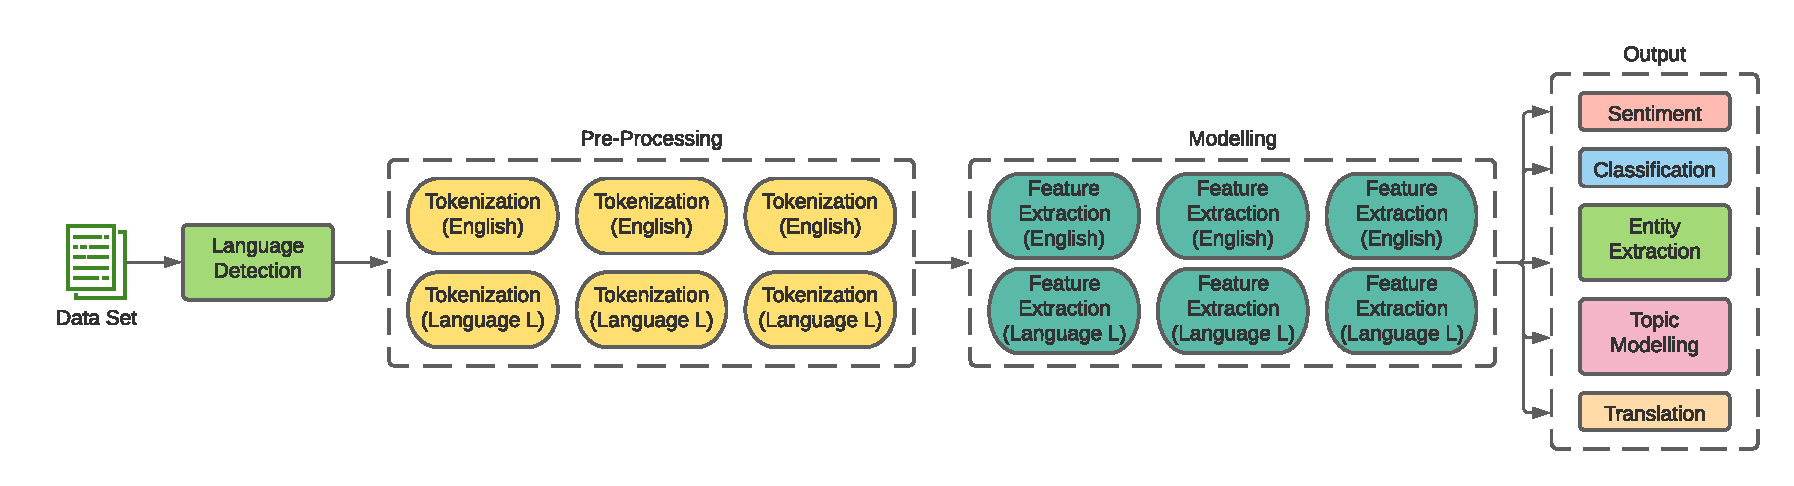
\includegraphics[width=\textwidth]{figures/chapter-5/ClassicalNLP.pdf}
    \caption[ClassicalNLP]{Classical NLP pipeline for text classification.
    \label{fig:ClassicalNLP}}
\end{figure}

Classical or "traditional" methods for corpus classification include: N-Grams, Hidden Markov Models using Markov Chains, Part-Of-Speech Tagging and Bag-Of-Words. Machine learning concepts can be classed as a “black-box” of functionality as the user does not necessarily see what is being executed within the hidden layers, a high-level abstraction for this project can be generalised into the following diagram:

\begin{figure}[H]
    \centering
    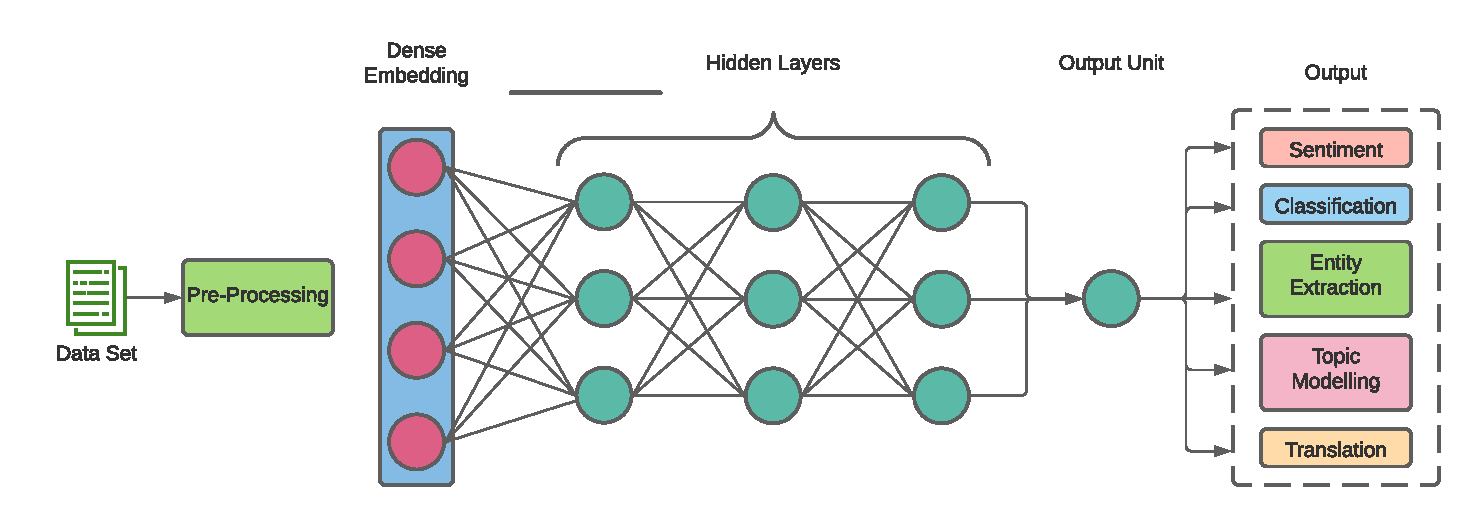
\includegraphics[width=\textwidth]{figures/chapter-5/MLNLP.pdf}
    \caption[MachineLearningNLP]{Machine Learning Model for an NLP pipeline for text classification.
    \label{fig:MLNLP}}
\end{figure}

\subsection{Model Approach --- Traditional}

The traditional implementation would have been designed based on word-embeddings within a 2D space where word vector values would be used alongside the Bag-Of-Words approach. The combination of Bag-Of-Words with a machine learning model to calculate a word’s vector based on its TF-IDF value would have been the start, such that:

\begin{equation}
    tf(t,d) = \frac{f_t, _d}{\sum{t \in_d} f _t {_`}, _d}
\end{equation}

Where the TF-IDF value is how often a lexeme occurs in a given corpus and would have also used the inverse TF-IDF value as the project model covers multiple datasets, such that:

\begin{equation}
    idf(t, D) = \log \frac{N}{|d \in D : t \in d|}
\end{equation}

Where the inverse TF-IDF value is represents how rare a word is in a given corpus.

\subsection{Limitations of Bag-Of-Words}

As there is a specific domain for this project, it is important to focus on the limitations for potential methods, CBOW models have demonstrated high training accuracy and is a relatively simple model to implement, it is naturally flexible as it can be trained on different datasets for a specific context; however, it does have disadvantages for classification and text prediction. Universities host students from different backgrounds and levels of education which can imply issues when training datasets, these issues can impact: the

\begin{itemize}
    \item \textbf{\textit{Vocabulary:}} Students may have varying output to describe the same context, this can create confusion for training.
    \item \textbf{\textit{Frequency:}} The frequency of a word may influence its power in a dataset.
    \item \textbf{\textit{Context:}} If students describe the same situation in a different way, some words may lose semantic meaning or be interpreted incorrectly, for example isolating neologisms, synonyms, colloquialism, or semantic change.
\end{itemize}

\subsection{Model Approach --- Modern}

Modern or "contemporary" methods for corpus classification include: \ldots The modern implementation would have been based around Word2Vec implemented in a machine learning model for Sentiment Analysis which can be seen as a subcategory of text classification. The word2vec implementation would produce vector values for identified key words and plot them as such:

\begin{figure}[H]
    \centering
    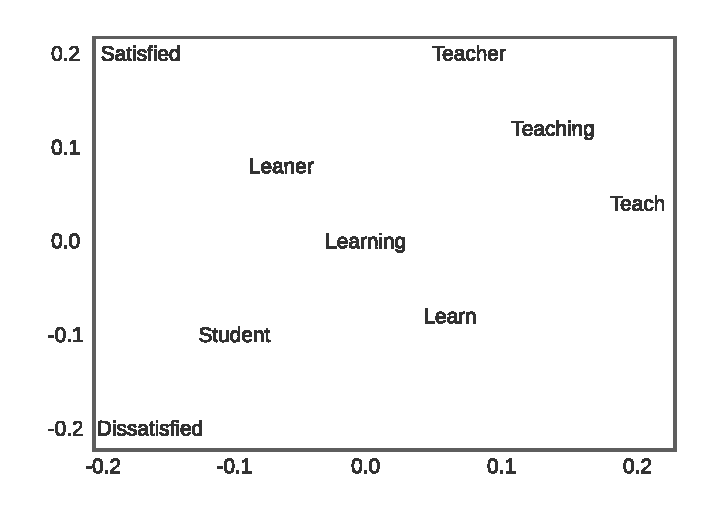
\includegraphics[width=\textwidth]{figures/chapter-5/Example-Word-Vector.pdf}
    \caption[ExampleWordVector]{Example of student satisfaction vector.
    \label{fig:Example-Word-Vector}}
\end{figure}

\subsection{Word2Vec Skip-Gram}

Skip-gram rather than Continuous Bag-Of-Words (CBOW [which is the modern implementation of Bag-Of-Words]) as it yields better results with large datasets - such as student feedback - skip gram can also be context aware as it converts neighboring lexemes to vectors.

\begin{figure}[H]
    \centering
    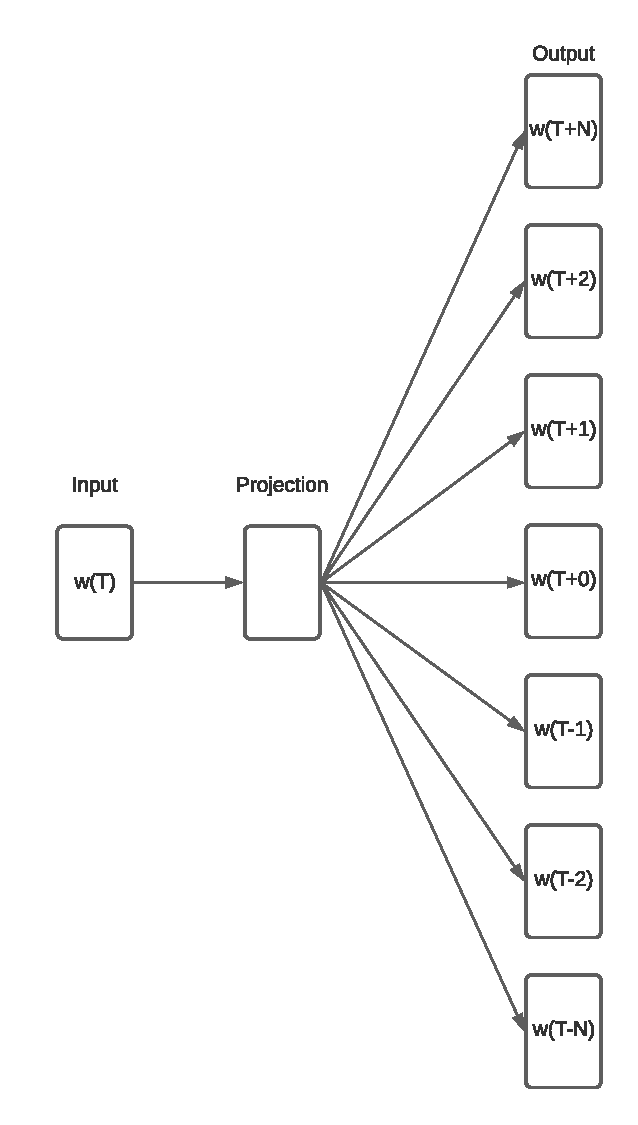
\includegraphics[width=0.49\textwidth]{figures/chapter-5/SkipGramModel.pdf}
    \caption[SkipGramModel]{Input flow of Skip-Gram model.
    \label{fig:SkipGramModel}}
\end{figure}

The skip-gram model can be seen as the inverse of the bag-of-words model as it attempts to vectorize neighboring words first to identify corpus context, whereas, bag-of-words takes each lexeme first, produces a vector sum and then categorises each word.

\begin{figure}[H]
    \centering
    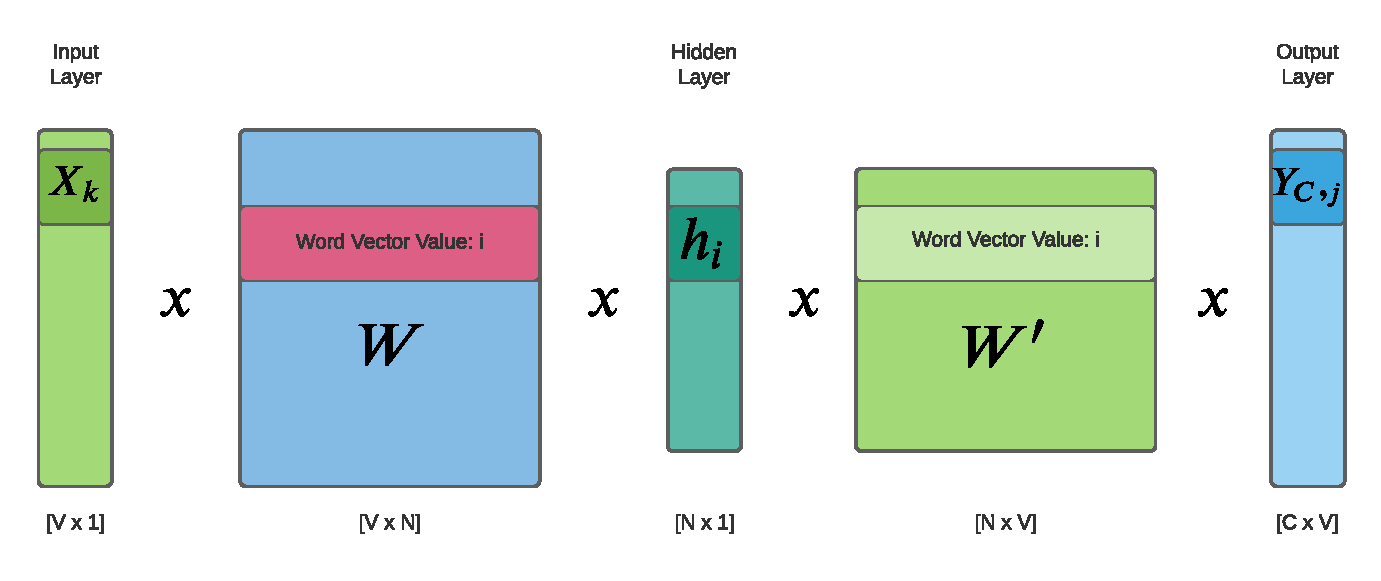
\includegraphics[width=\textwidth]{figures/chapter-5/SkipGramNetwork.pdf}
    \caption[SkipGramNetwork]{Skip-Gram implementation for Word2Vec network architecture.
    \label{fig:SkipGramNetwork}}
\end{figure}

The Skip-Gram's network architecture is similar to the diagram displayed in \autoref{fig:MLNLP}, the diagram above is another level of abstraction as to how this project will make use of machine learning fundamentals.

\subsection{One-Hot Encoding}

Encoding each important lexeme in a given dataset is helpful for the model to distinguish the level of importance, outlined as context, the diagram shown above in \autoref{fig:SkipGramModel} takes a 1D vector matrice as the input layer which allows for the model to acceptably one-hot encode each lexeme datum as a numeric value.

\begin{multicols}{2}
    \begin{equation*}
        Teach =
        \begin{bmatrix}
            0 & 0 & 0 & 0 & 1 & 0
        \end{bmatrix}
    \end{equation*}

    \begin{equation*}
        Teaching =
        \begin{bmatrix}
            0 & 0 & 0 & 0 & 1 & 0
        \end{bmatrix}
    \end{equation*}
\end{multicols}

This equates to differing versions of the same word to have the same influence when training the mode.

\subsection{Forward Passes}

\begin{equation}
    h = x^T W
\end{equation}


\begin{equation}
    h = W_{(k,:)}^{T} \coloneqq v_{w_I}^{T}
\end{equation}


\begin{equation}
    u_{c} = W'^{T}h = W'^{T} W^{T}x
\end{equation}


\begin{equation}
    y_{c} = Softmax(u)
\end{equation}


\begin{equation}
    p(w_{c,_j} = w_{O,_c} | w_{I}) = y_{c,_j} = \frac{exp(u_{c_j})}{\sum_{j' = 1}^{V} exp(u_{j'})}
\end{equation}


\begin{equation}
    u_{c,_j} = u_{j} = {v'_{w_j}} ^ T \cdot h
\end{equation}

\subsection{Backpropagation}

% Needs remaking
% \begin{equation} \label{}
%     \begin{split}
%         Er & = - \log \mathbb{P} (w_O_,{_1} , \ldots, w_O_,{_c} | w_{I}) \\
%            & = - \log \prod_{c=1}^{C} \frac{exp(u_c,_{j_{c}^{*}})}{\sum_{j'=1}^{V} exp(u_j')} \\
%            & = - \sum_{c=1}^{C} u_{j_{c}^{*}} + C \cdot \log \sum_{j'=1} ^ {V} exp(u_j_')
%     \end{split}
% \end{equation}

\section{Planning the ML Model Design}

Initial prototyping of the machine learning model for a new amalgamation of NLP techniques helped to indicate what the best route of development could be, the planning stage piggybacked off existing work flowchart diagrams in-order to apply the most appropriate method and technique combination. The sequence flowchart is as follows:

\begin{figure}[H]
    \centering
    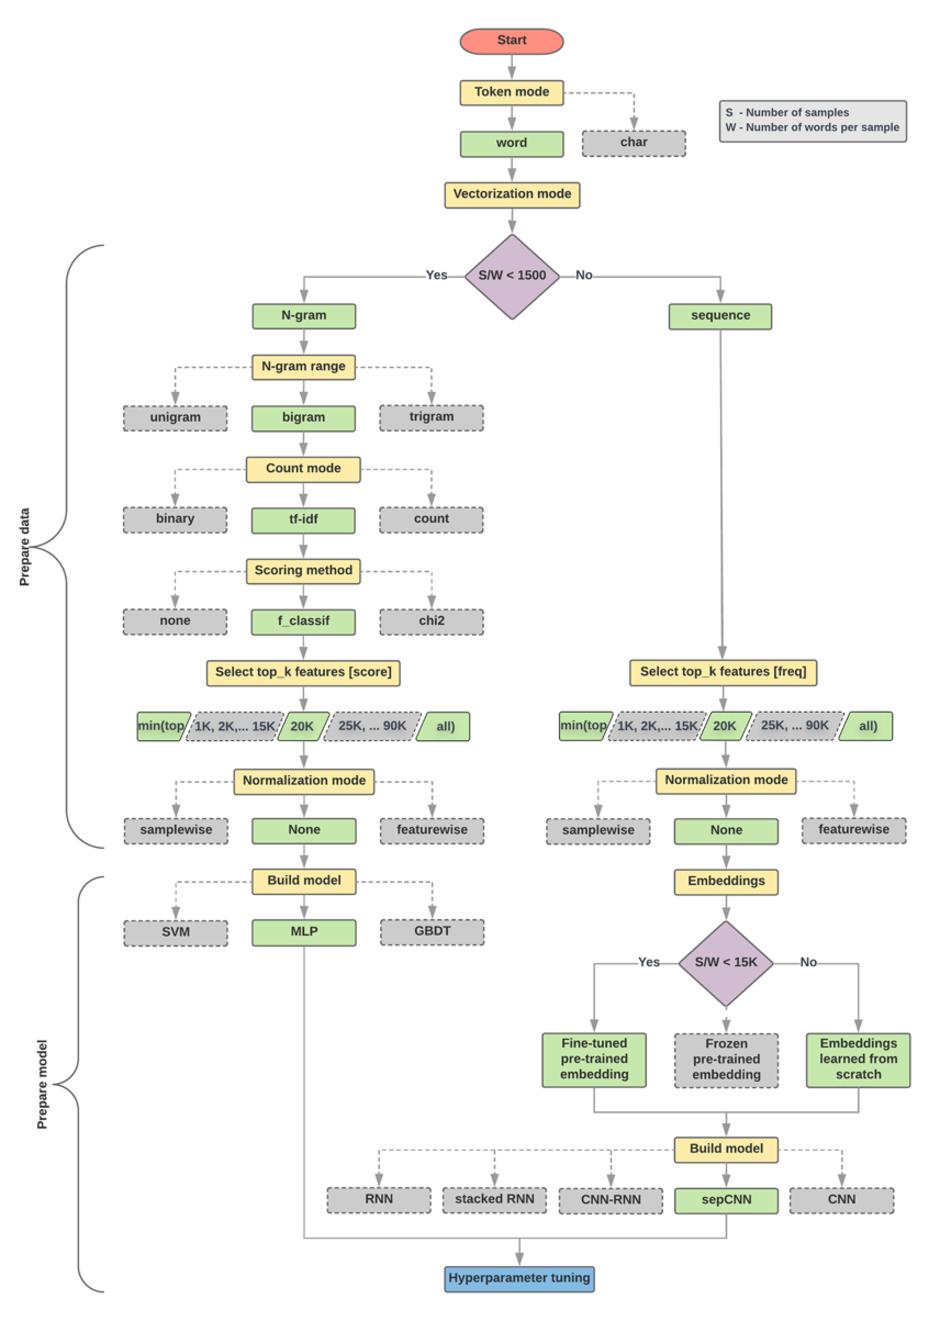
\includegraphics[width=\textwidth]{figures/chapter-5/GooglePlan.pdf}
    \caption[GooglePlan]{Text Classification Flowchart \parencite{google2021TCF}.
    \label{fig:GooglePlan}}
\end{figure}

\section{Supervision}

The development of the project model is based on a supervised approach due to the datasets located, it was most appropriate to use a supervised approach due to the datasets having no labels or lexical categories to train the model on; the model has user input to account for missing labels on data which have been manually and algorithmically added. The supervision for this project can be represented as the following diagram:

\begin{figure}[H]
    \centering
    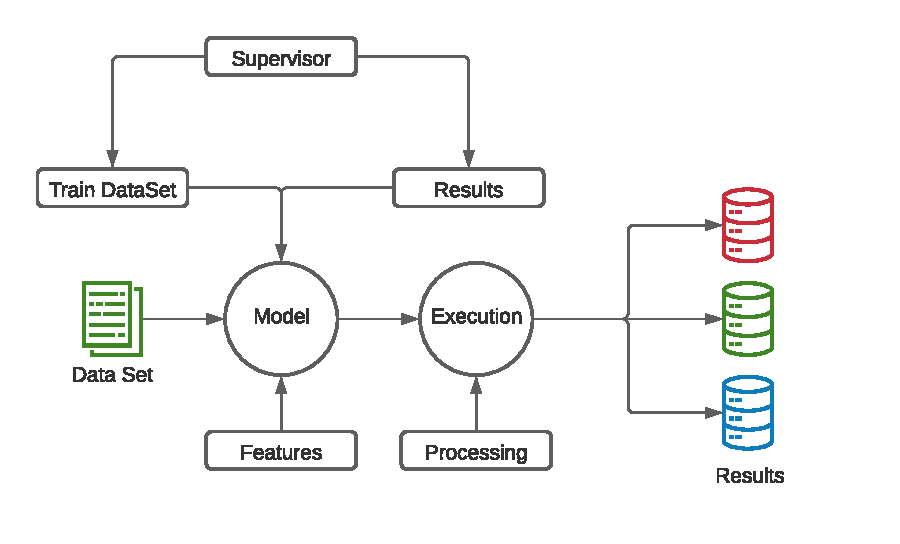
\includegraphics[width=\textwidth]{figures/chapter-5/SupervisedLearningChart.pdf}
    \caption[SupervisedLearning]{Sequence control for Supervised learning.
    \label{fig:SupervisedLearningChart}}
\end{figure}

\section{Pipeline Design}

\begin{figure}[H]
    \centering
    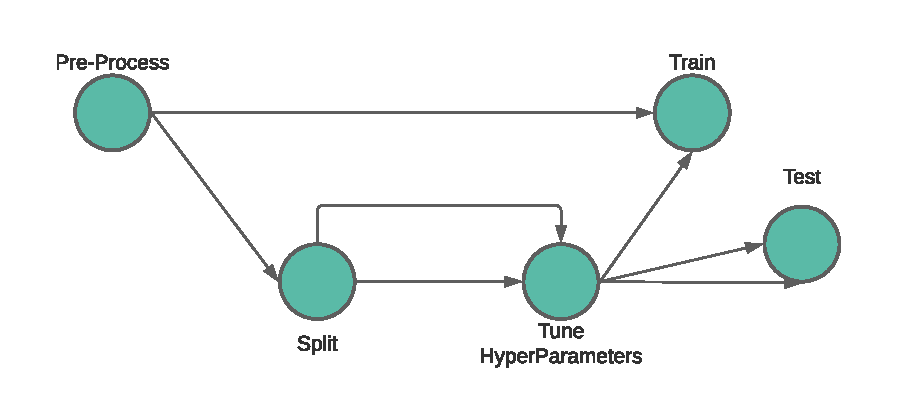
\includegraphics[width=\textwidth]{figures/chapter-5/Pipeline.pdf}
    \caption[MLTCPipeline]{Pipeline for model classification.
    \label{fig:MLTCPipeline}}
\end{figure}

There are five main steps for a text classification pipeline:

\begin{enumerate}
    \item \textbf{\textit{Pre-processing}}: prepare the raw dataset to be trained.
    \item \textbf{\textit{Splitting}}: split the processed dataset to be trained and validated.
    \item \textbf{\textit{Tuning}}: identity valuable parameters within trained data.
    \item \textbf{\textit{Training}}: train the current iteration of the model with updated hyper-parameters.
    \item \textbf{\textit{Testing}}: test and collect statistics for analysis to make further predictions.
\end{enumerate}

\section{Data Preparing and Pre---processing}

Data Preparing